\documentclass[11pt]{article}
\usepackage{amsmath, amsfonts, amsthm, amssymb}  % Some math symbols
\usepackage{mathtools} % defines \coloneqq
\usepackage{enumerate}
\usepackage{fullpage}
\PassOptionsToPackage{normalem}{ulem}
\usepackage{ulem}
\usepackage{url}
\usepackage{hyperref}

\usepackage[x11names, rgb]{xcolor}
\usepackage{tikz}
\usepackage{graphicx}

\setlength{\parindent}{0pt}
\setlength{\parskip}{5pt plus 1pt}
\pagestyle{empty}

\def\indented#1{\list{}{}\item[]}
\let\indented=\endlist

\newcounter{questionCounter}
\newcounter{partCounter}[questionCounter]

\newenvironment{question}[2][\arabic{questionCounter}]{%
    \addtocounter{questionCounter}{1}%
    \setcounter{partCounter}{0}%
    \vspace{.25in} \hrule \vspace{0.5em}%
        \noindent{\bf #2}%
    \vspace{0.8em} \hrule \vspace{.10in}%
}{}

\renewenvironment{part}[1][\alph{partCounter}]{%
    \addtocounter{partCounter}{1}%
    \vspace{.10in}%
    \begin{indented}%
       {\bf (#1)} %
}{\end{indented}}

% ----- Identifying Information -----------------------------------------------
\newcommand{\myclass}{16-722}
\newcommand{\myname}{Wei Liang}
\newcommand{\myandrew}{weiliang@andrew.cmu.edu}
\newcommand{\myhwname}{Assignment 1}
\newcommand{\myrecitation}{Section A}
% -----------------------------------------------------------------------------

\begin{document}
\begin{center}
  {\Large \myclass{} \myhwname} \\
  \myname \\
  \myandrew \\
  \myrecitation \\
  \today
\end{center}

% ----- Your Content (delete from here until \end{document}) ------------------

% Example Usage
\begin{question}{Problem 1}
    \begin{part}
        People talking at the restaurant table next to yours can be technical noise if you are listening to people talking to you at your own table. It can be avoided by moving to another table that are farther to people talking at the restaurant table next to yours. However, people talking at the restaurant table next to yours can be a signal if you get interested and pay attention to their conversion intentionally.
    \end{part}
    \begin{part}
        Earth tide can be technical noise when measuring ground water levels. It can caused periodic disturbances. Earth tide noise can be reduced using regression deconvolution \cite{tide}. However, earth tide can be a signal if you are aiming to measure oscillation of the the displacement of the solid earth’s surface due to the gravity of the Moon and Sun.
    \end{part}
    \begin{part}
        Reflections in a ship’s sonar system due to fish is a kind of technical noise. Since the sonar system utilizes sound waves for detection underwater, the distribution and vocalization of fish will affect the performance of the sonar system. The magnitude, randomness, and spatial distribution of the noise caused by fish can be estimated by mathematical models for noise reduction \cite{fish}. It is unlikely Reflections in a ship’s sonar system due to fish since in this set-up the sonar system is for navigation. However, there are sonar systems designed for detection of fish schools, then the reflections in a ship’s sonar system due to fish will be a signal.
    \end{part}
    \begin{part}
        Vibrations recorded by an interferometer due to footsteps outside the lab is technical noise. It cannot be a signal since interferometer is not used for detecting footsteps. The technical noise can reduced by stabilization of the equipment.
    \end{part}
    \begin{part}
        It is Johnson noise, one kind of intrinsic noise. Johnson noise is temperature-dependent voltage, and it has a zero means. However, the RMS is not zero as $V^2$ is not zero, which matches the description of the problem.
    \end{part}
    \begin{part}
        It is $1/f$ noise, one kind of intrinsic noise. The example is a case of low frequency, and it exhibits generally increasing amplitudes at longer periods. This description matched the characteristics of $1/f$ noise, also called pink noise.
    \end{part}
\end{question}

\begin{question}{Problem 2}
  A line spectrum is a signal formed by only one single line pf a particular wavelength.
  
  A continuum spectrum is a signal consist of a continuous set (certain bandwidth) of wavelengths.
  
  In real-world, a line spectrum is not truly a line spectrum, but rather a narrow-bandwidth continuum spectrum because there is no real impulse function in the real-world. Any line or point still has an finite amount of continues values but it is just too narrow to observe in real-world. 
\end{question}

\begin{question}{Problem 3}
According to the description, without considering the initial phase, the time domain response of the system can be written as:
\begin{align*}
    h(t) &= e^{-\alpha t}cos(\omega t) \\
    &= e^{-\alpha t}cos(2 \pi f t) \\
    &= e^{-\frac{1}{600}t}cos(20 \pi t)
\end{align*}
Using Laplace transform, the frequency transfer function is
\begin{equation}
    H(s) = \frac{s + \frac{1}{600}}{(s+\frac{1}{600})^2 + (20\pi)^2} = \frac{s + \frac{1}{600}}{s^2 + \frac{1}{300}s + (\frac{1}{36000}+400\pi^2)}
\end{equation}
Using MATLAB, we can have the bode plot for its frequency response:
\begin{figure}[ht]
    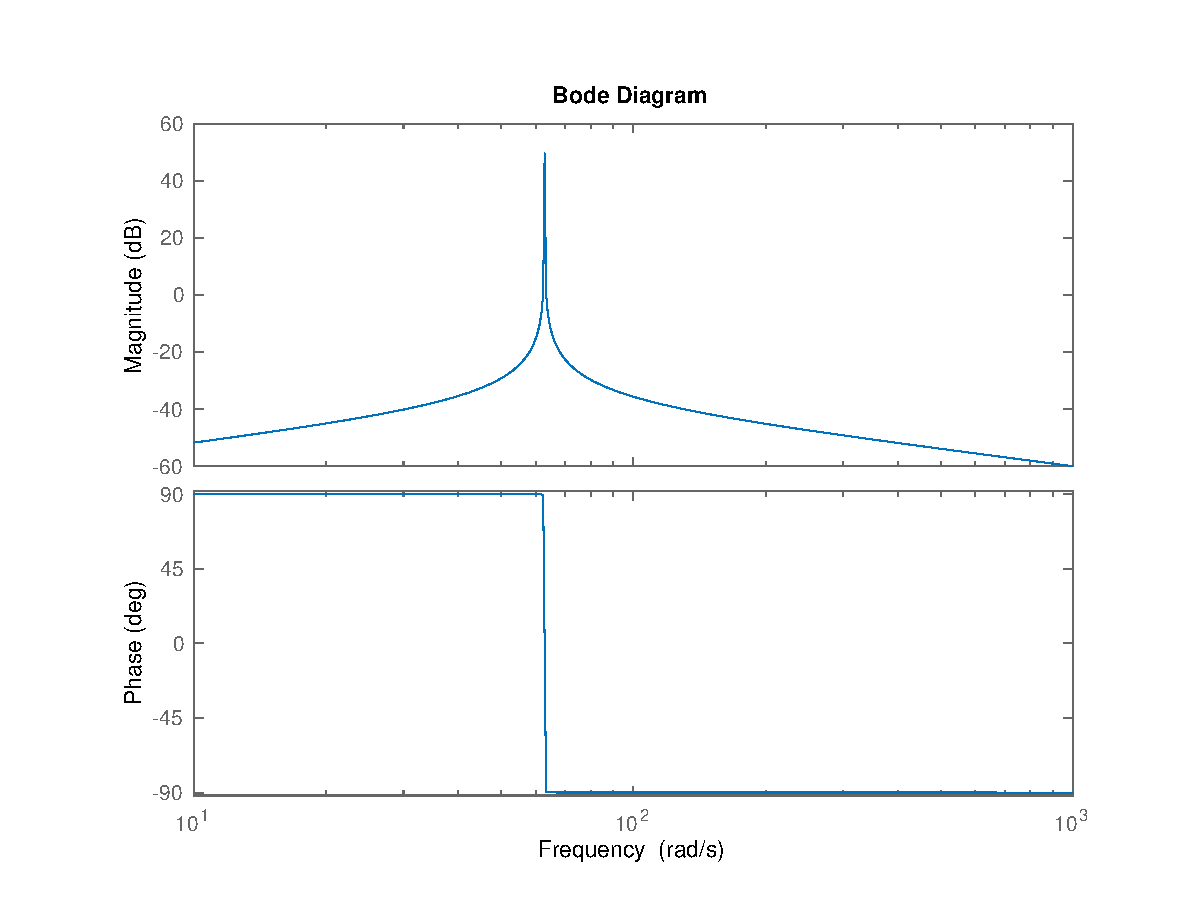
\includegraphics[width=12cm]{p3.eps}
    \centering
\end{figure}
We can see the effect of the damping to the system, but based on the definition of cutoff frequencies, the frequency spectrum of this system can still consider as a line spectrum at 10 Hz. 
\end{question}

\begin{question}{Problem 4}
    The name \textit{white noise} is from the white light. As white light is composed of "all colors" with the same magnitude, as white noise consists of same power at all frequencies.
    
    The name \textit{pink noise} is from the pink light, as more power toward “red” at end of spectrum, as the magnitude of the noise decays when the frequency rises up. 
    
    The name \textit{brown noise} is from Brownian motion. Power even greater toward “red” end of spectrum, as as the magnitude of the noise decays even faster than the pink noise when the frequency rises up.
\end{question}

\begin{question}{Problem 5}
The current is $10$ mA $= 0.01$ A, and bandwidth is $1$ MHz $= 1 \times 10^{6}$ Hz. According to the equation of shot noise, we have:
\begin{equation*}
    \sigma_{I} = \sqrt{2e\Bar{I}\Delta f} = \sqrt{2 \times 1.602 \times 10^{-19} c \times 0.01 A \times 1 \times 10^{6} Hz} = 5.6604 \times 10^{-8} A
\end{equation*}
The current noise is $5.6604 \times 10^{-8}$ A $= 5.6604 \times 10^{-5}$ mA.
\end{question}

\begin{question}{Problem 6}
    At room temperature, $4kT \approx 1.6 \times 10^{-20} J$. The bandwidth of human hearing is  $\Delta f = 20 kHz - 20 Hz \approx 20 kHz$. Thus,
 \begin{equation*}
    V_{noise} = \sqrt{4kTR\Delta f} = \sqrt{1.6 \times 10^{-20} J \times 10^4 \Omega \times 2 \times 10^4 Hz} = 1.8 \times 10^{-6} V
    \end{equation*}   
The RMS voltage noise is $1.8 \times 10^{-6}$ V $= 1.8 \times 10^{-3}$ mV.
\end{question}

\begin{question}{Problem 7}
For the least-significant fluctuation of a 10-bits ADC/5V system, the amplitude is:
\begin{equation*}
    V_{1-bit} = \frac{5}{1023} \approx 4.9 \times 10^{-3} V
\end{equation*}
We know that for an RC circuit $\omega = 2\pi\Delta f = \frac{1}{RC}$, so $\Delta f = \frac{1}{2\pi RC}$. For the Johnson noise of the resistor in the RC circuit, we have
\begin{align*}
    &V_{noise} = \sqrt{4kTR\Delta f} \\
    \Longrightarrow& T = \frac{V_{noise}^2}{4kR\Delta f} = \frac{V_{noise}^2}{4kR \frac{1}{2\pi RC}} = \frac{\pi V_{noise}^2 C}{2k}
\end{align*}
In this problem, $V_{noise} = V_{1-bit}$, so $T = \frac{\pi V_{1-bit}^2 C}{2k} =\frac{3.14 \times (4.9 \times 10^{-3} V)^2 \times 100 \times 10^{-12} F}{2 \times 1.38064852 \times 10^{-23} \frac{m^2 kg}{s^2 k}} \approx 27.3 \times 10^{7} K$. The temperature is impossible to achieve under normal conditions. It means that the Johnson noise of the resistor under normal condition cannot be picked up by the Arduino system.
\end{question}

\begin{question}{Problem 8}
First of all, drift is a kind of extrinsic noise that can be reduced or eliminated by techniques as chopper stabilization \cite{chopper}, while 1/f noise is a kind of intrinsic noise.

The reason of 1/f noise is still an active research area, but drift can cause by different problems, such as the electric field, the aging of the resistance. Also, different types of drift have different patterns, as some drift may be temperature-dependent, and drift caused by aging is more linear. For 1/f noise, the pattern is ‐3 dB per octave.

It is believed that the drift mechanisms is fundamentally different to that of 1/f noise. 

In low frequencies, 1/f noise is difficult to be distinguished from drift \cite{dist}. 

\end{question}
% -----------------------------------------------------------------------------

\begin{thebibliography}{1}
\bibitem[1]{tide} Toll, Nathanial J and Rasmussen, Todd C. ``Removal of barometric pressure effects and earth tides from observed water levels,'' \emph{Groundwater}, 2006. Link: \label{et}\emph{\uline{https://doi.org/10.1111/j.1745-6584.2006.00254.x}}. 

\bibitem[2]{fish} Newcombe, Richard A., et al. ``Estimation and simulation of multi-beam sonar noise.'' \emph{The Journal of the Acoustical Society of America}, 2016. Link: \label{es}\emph{\uline{https://doi.org/10.1121/1.4941913}}.

\bibitem[3]{chopper} Gregorian, Roubik, and Gabor C. Temes. \emph{Analog MOS integrated circuits for signal processing}, 1986, Wiley-Interscience.

\bibitem[4]{dist} Klumperink, Eric AM, et al. ``Reducing MOSFET 1/f noise and power consumption by switched biasing.'' \emph{IEEE Journal of Solid-State Circuits}, 2000. Link: \label{es}\emph{\uline{https://ieeexplore.ieee.org/document/1471119}}.
\end{thebibliography}
\end{document}
